The soft background component is suppresed by a lead shield inside which the TRITIUM detector is placed. This lead shield is efficient for suppressing particles with energies below $200~\MeV$, that originate from the Earth's natural radioactivity and the soft component of cosmic radiation. This lead shield consists of $158$ low intrinsic radioactivity lead bricks of $25~\mm$ thickness. The bricks are chevron shaped, as shown in Figure \ref{fig:LeadBrick}, specially designed for a perfect fit and easy assembly. As can be seen in Figures \ref{subfig:TwoLayers} and \ref{subfig:TwoLayers2}, these lead bricks are arranged in two layers with a total thickness of $50~\mm$. 

\begin{figure}[h]
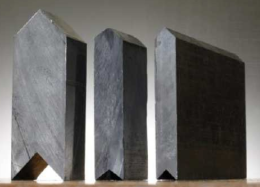
\includegraphics[scale=0.6]{3DesignPrinciples/34BackgroundRejectionSystem/LeadBricks.png}
\centering
\caption{Lead bricks.\label{fig:LeadBrick}}
\end{figure}

\begin{figure}[h]
\centering
    \begin{subfigure}[b]{0.5\textwidth}
    \centering
    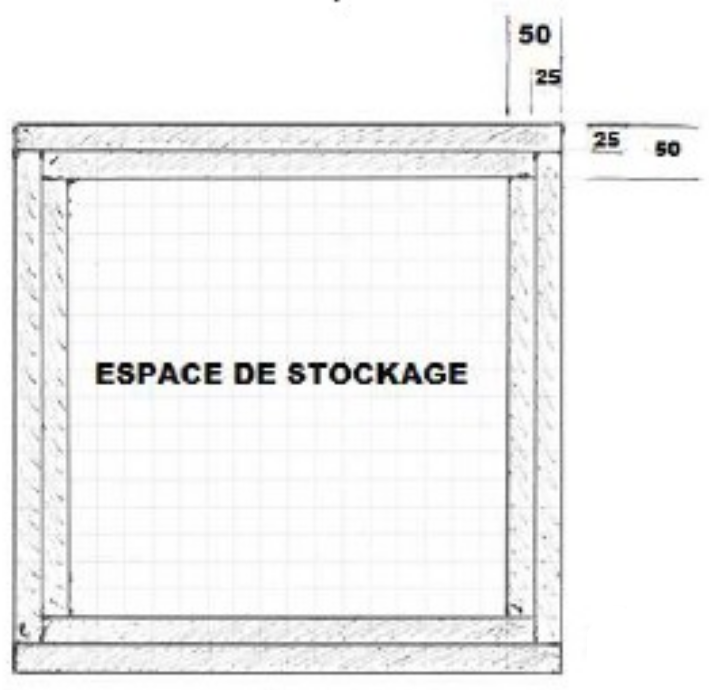
\includegraphics[width=\textwidth]{3DesignPrinciples/34BackgroundRejectionSystem/TwoLayers.png}  
    \caption{\label{subfig:TwoLayers}}
    \end{subfigure}
    \hfill
    \begin{subfigure}[b]{0.4\textwidth}
    \centering
    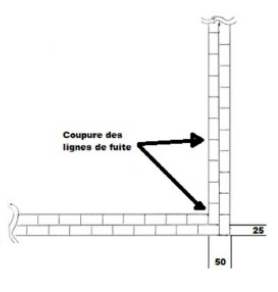
\includegraphics[width=\textwidth]{3DesignPrinciples/34BackgroundRejectionSystem/TwoLayers2.png}  
    \caption{\label{subfig:TwoLayers2}}
    \end{subfigure}
 \caption{Two layers for the lead bricks of the shield.}
 \label{fig:LeadBricksAndArrangement}
\end{figure}

An aluminium structure capable of supporting the total weight of $2.4$ tons of lead bricks, shown in Figure \ref{fig:AluminiumStructure}, was designed by the Mechanical Engineering Department of the CENBG.

\begin{figure}
\centering
    \begin{subfigure}[b]{0.5\textwidth}
    \centering
    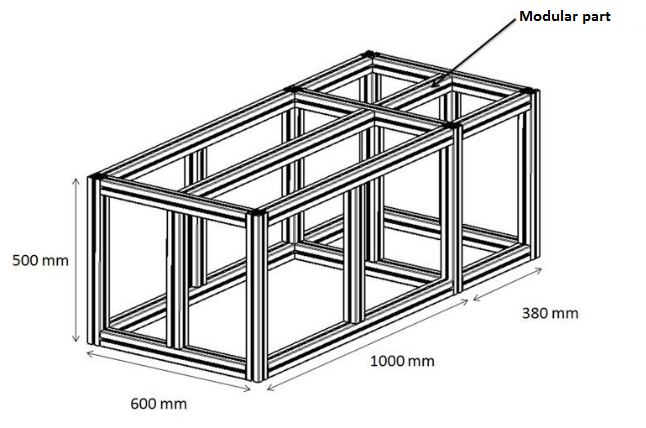
\includegraphics[width=\textwidth]{3DesignPrinciples/34BackgroundRejectionSystem/AluminiumStructureScheme.png}  
    \caption{\label{subfig:AluminiumStructureScheme}}
    \end{subfigure}
    \hfill
    \begin{subfigure}[b]{0.45\textwidth}
    \centering
    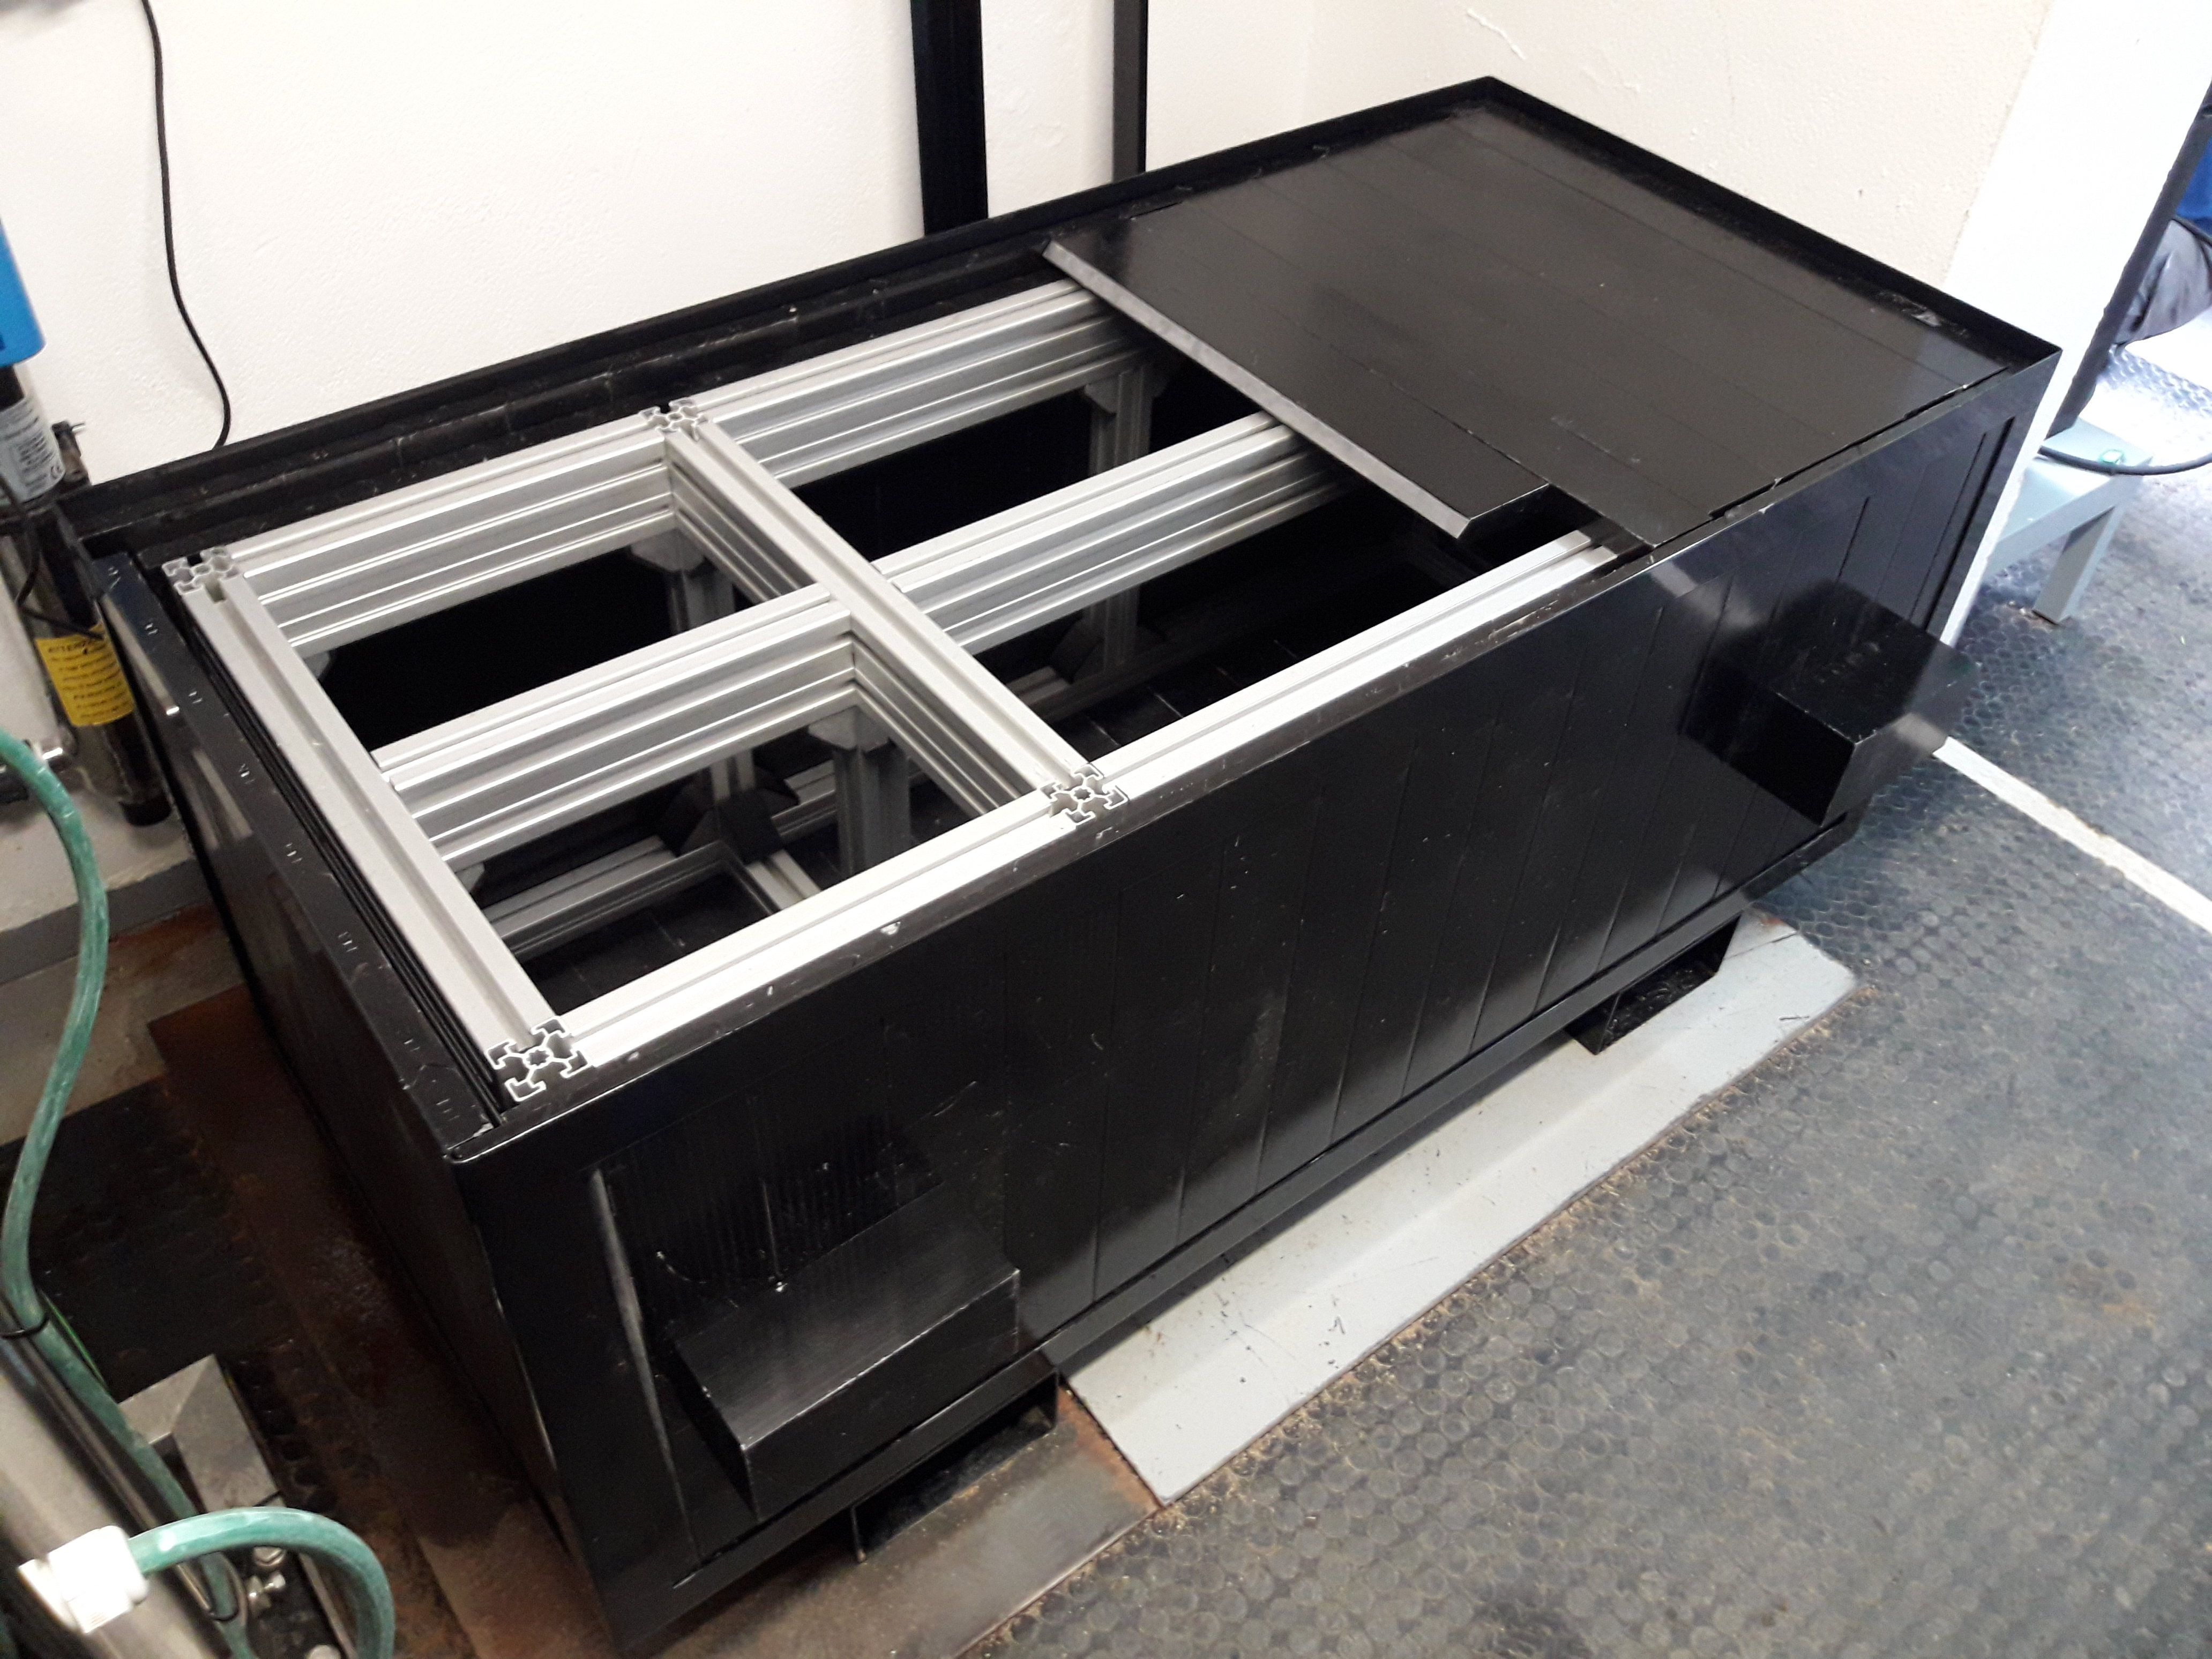
\includegraphics[width=\textwidth]{3DesignPrinciples/34BackgroundRejectionSystem/AluminiumStructure.jpg}  
    \caption{\label{subfig:AluminiumStructure}}
    \end{subfigure}
    \caption{a) Scheme of the aluminium structure of the shield. b) The lead shield partially mounted.}
 \label{fig:AluminiumStructure}
\end{figure}

The internal room of the lead shield is divided into two parts, as indicated in Figure \ref{fig:AluminiumStructure}. The larger one has internal dimensions of $90.5 \times 41 \times 51~\cm^3$ and is used to place the TRITIUM detector. The smaller one, of dimensions of $33 \times 41 \times 51~\cm^3$, contains the DAQ system of the detector. The external dimensions of the lead shield are $148 \times 60 \times 70~\cm^3$ and its total weight is $2.5$ tons.